\documentclass[12pt]{article}

% Packages
\usepackage{lastpage} 
\usepackage{fancyhdr}	%For header and footer
\usepackage{amsmath, amsthm, amssymb} %For mathematics
\usepackage{graphicx}
\usepackage{hyperref}	%For hyperlinks

% Page setup
\setlength{\topmargin}{-0.4in}
\setlength{\topskip}{0.3in}    % between header and text
\setlength{\textheight}{9.in} % height of main text
\setlength{\textwidth}{6.5in}    % width of text
\setlength{\oddsidemargin}{0in} % odd page left margin
\setlength{\evensidemargin}{0in} % even page left margin
\setlength{\parindent}{0pt}	% Suppress the indent

% Macros
\newcommand*{\bv}[1]{\textbf{#1}} % Write vectors in bold case within an equation environment

% Header and Footer
\pagestyle{fancy}%\fancyhead{}
\fancyhf{}	% Clear the default header and footer
\fancyhead[L]{MAE 3195 \\ Name:}
\fancyhead[R]{Credit Sheet 12 \\ \thepage /\pageref{LastPage}}


% Title
\title{MAE 3195, Credit Sheet 12\\
Optimization}
\date{}

% Body of document
\begin{document}
\maketitle

For this homework, you will design an optimum box. The design parameters of the box are shown in the figure below. All of the box's walls have uniform thickness, $t = 5$ mm. The box is to fit on a 18 inch deep shelf that is only 8 feet long. The distance in between shelves is only 18 inches. The box is made of PVC, and the specific cost (cost per unit mass) of this material is $C$~= ~\$0.25 per kg. Find the dimensions of the least expensive box that has at least 0.1~m$^3$ of storage space.

\begin{figure}[htp]
  \begin{center}
    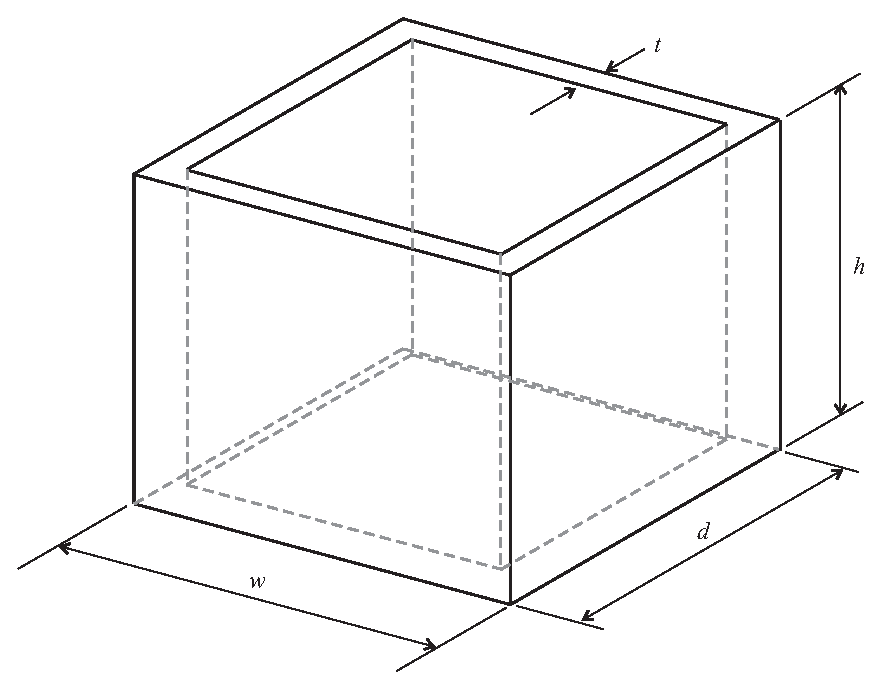
\includegraphics[width=6.in]{box_CS12}
    %\caption{Geometry for question 5}
    \label{figBox}
  \end{center}
\end{figure}


\pagebreak

\section*{Review Questions}
\begin{enumerate}
	\item What are the design parameters for this design problem?
	\vspace{1.25in}
	\item What are the valid ranges for the design parameters?
	\vspace{1.25in}
	\item What other constraints are required?
	\vspace{1.25in}
	\item What is the objective function?
	\vspace{1.25in}
	\item List and describe each feature that you built in Pro/Engineer.
	\pagebreak
	\item List and describe each entry in the Optimization/Feasibility window (Goal, Design Constraints, Design Variables) in Pro/Engineer.
	\vspace{2.5in}
	\item What are the dimensions of the optimal box?
	\vspace{1.25in}
	\item What is the cost of the optimal box?
	\vspace{1.25in}
	\item Would you expect different results from the optimization if you were minimizing the weight of the box? Why?
\end{enumerate}

\end{document}